\section{OpenSHMEM Memory Model}
\label{src:mmodel}
\begin{figure}[!h]
    \vspace{-30pt}
    \hspace*{5mm}
    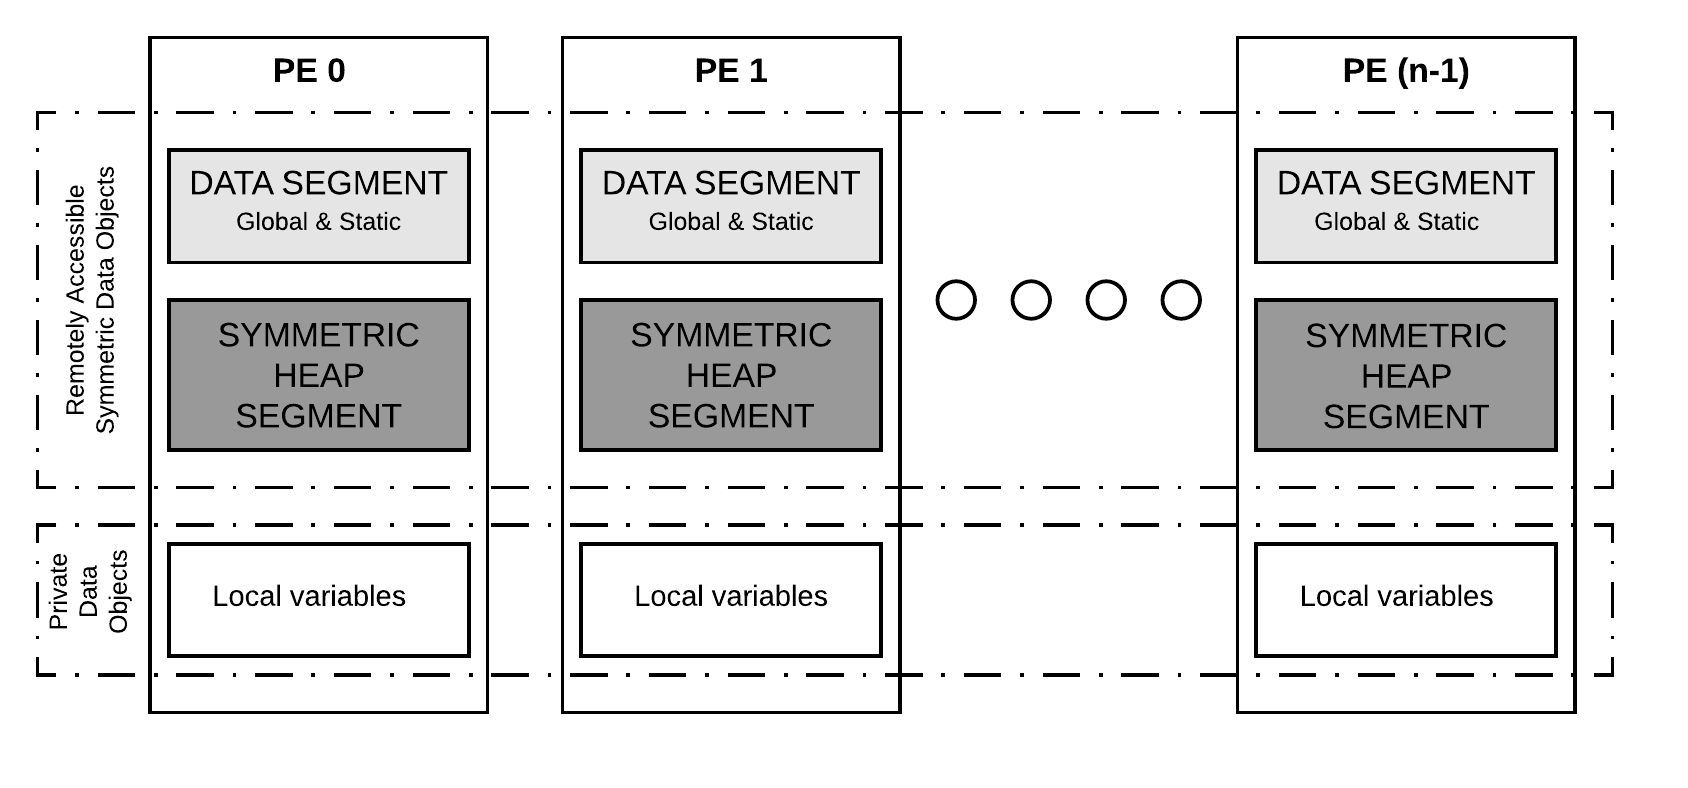
\includegraphics[scale=0.20]{image/osm-mmodel.png}
    \vspace{-25pt}
    \caption{OpenSHMEM Memory Model}
    \vspace{-20pt}
    \label{fig:mmodel}
\end{figure}

OpenSHMEM program consists of two types of data objects: remotely
accessible and private data objects. The private data objects are local
to a particular PE and are accessible by only that PE. It follows the
same memory model of the base programming language (C or Fortran). The
remotely accessible data objects are accessible by any PE using the
OpenSHMEM routines and are called as \emph{Symmetric Data Objects}.
Each symmetric data object has a corresponding object with same variable
name, size and data type on all PEs and the following variables are
considered as Symmetric Data Objects:
\begin{itemize}
    \item global or static variable on C/C++ and not defined in DSO; and
    \item data allocated by \texttt{shmem\_malloc} OpenSHMEM routines.
\end{itemize}

The data allocated by \texttt{shmem\_malloc} collective OpenSHMEM
routines are placed on a special memory region called \emph{Symmetric
Heap}. There is one symmetric heap on every PE created during the program
execution on a memory region determined by the OpenSHMEM implmentation.
It may reside on different memory regions on different PEs. Except the
size of the symmetric heap determined by \texttt{SMA\_SYMMETRIC\_SIZE}
environment variable, users have no other control on any property of
the symmetric heap.

Fig.~\ref{fig:mmodel}, shows the different types of data objects in
OpenSHMEM. Global and Static variables are allocated on the
\emph{data segment}, while the variables with data allocated using
\texttt{shmem\_malloc} routines are placed on the \emph{symmetric heap
segment}. Variables on both the data and symmetric heap segments are
remotely accessible. Fig.~\ref{fig:mmodel} also shows that there is only
one symmetric heap per PE. %Local variables are allocated on the local
%data objects which retains the same memory model from the underlying
%base language.

\subsection{Need for Heterogeneous Memory Support in OpenSHMEM}
\label{src:mmodel/drelated}
As mentioned in Section~\ref{src:knl/config}, MCDRAM in Intel KNL can be
configured either as cache or as addressable memory. While configuring as
cache is a convenient way to port existing applications on to KNL based
systems, it is more suitable only for applications that are optimized for
cache utilizations and with small memory footprint.

The flat mode configuration is suitable for memory bandwidth bound
applications. Taking advantage of the high bandwidth offered by MCDRAM by
making it available as a distinct NUMA node and re-designing an application
can improve the performance. Based on the MCDRAM utilization, memory
bandwidth bound applications are of two types:
\begin{itemize}
    \item applications where the entire memory can fit in the MCDRAM; and
    \item applications that are capable of partitioning memory usage into
    bandwidth critical and normal part, with the bandiwdth critical part
    allocated on MCDRAM.
\end{itemize}
The current OpenSHMEM memory model does not handle both the above mentioned
categories for utilizing MCDRAM in flat mode configuration. And it is not
for OpenSHMEM to handle anything special for cache mode configuration.
